% !TeX spellcheck = de_CH
%%%%%%%%%%%%%%%%%%%%%%%%%%%%%%%%%%%%%%%%%%%%%%%%%%%%%%%%%%%%%%%%%
%  _____   ____  _____                                          %
% |_   _| /  __||  __ \    Institute of Computitional Physics   %
%   | |  |  /   | |__) |   Zuercher Hochschule Winterthur       %
%   | |  | (    |  ___/    (University of Applied Sciences)     %
%  _| |_ |  \__ | |        8401 Winterthur, Switzerland         %
% |_____| \____||_|                                             %
%%%%%%%%%%%%%%%%%%%%%%%%%%%%%%%%%%%%%%%%%%%%%%%%%%%%%%%%%%%%%%%%%
%
% Project     : BA Welti Keller
% Title       : 
% File        : vorgehen.tex Rev. 00
% Date        : 15.09.2014
% Author      : Tobias Welti
%
%%%%%%%%%%%%%%%%%%%%%%%%%%%%%%%%%%%%%%%%%%%%%%%%%%%%%%%%%%%%%%%%%

\chapter{Vorgehen}\label{chap.vorgehen}
\section{Überblick}\label{sec.ueberblick}
Das zu entwickelnde Messsystem kann grob in drei Komponenten aufgeteilt werden. 
\begin{enumerate}
\item \gls{logger}
\item \gls{sensoreinh}
\item \gls{bussys}
\end{enumerate}
Der \gls{logger} hat die Aufgabe, von mehreren \glspl{sensoreinh} registrierte \glspl{ereignis} zu empfangen und zu speichern. Die \glspl{sensoreinh} messen kontinuierlich die Beschleunigung, werten die Signale aus und erkennen \glspl{ereignis}, die einer vordefinierten Signalform entsprechen. Alle \glspl{sensoreinh} sind über ein \gls{bussys} mit dem \gls{logger} verbunden, um miteinander kommunizieren zu können. Der prinzipielle Aufbau ist in Abbildung \ref{fig.situationskroki} ersichtlich. Die Stromversorgung der Anlage wird am \gls{logger} angeschlossen. Parallel zum Kabel des Datenbusses wird die Stromversorgung der \glspl{sensoreinh} geführt.

\begin{figure}
	\centering
		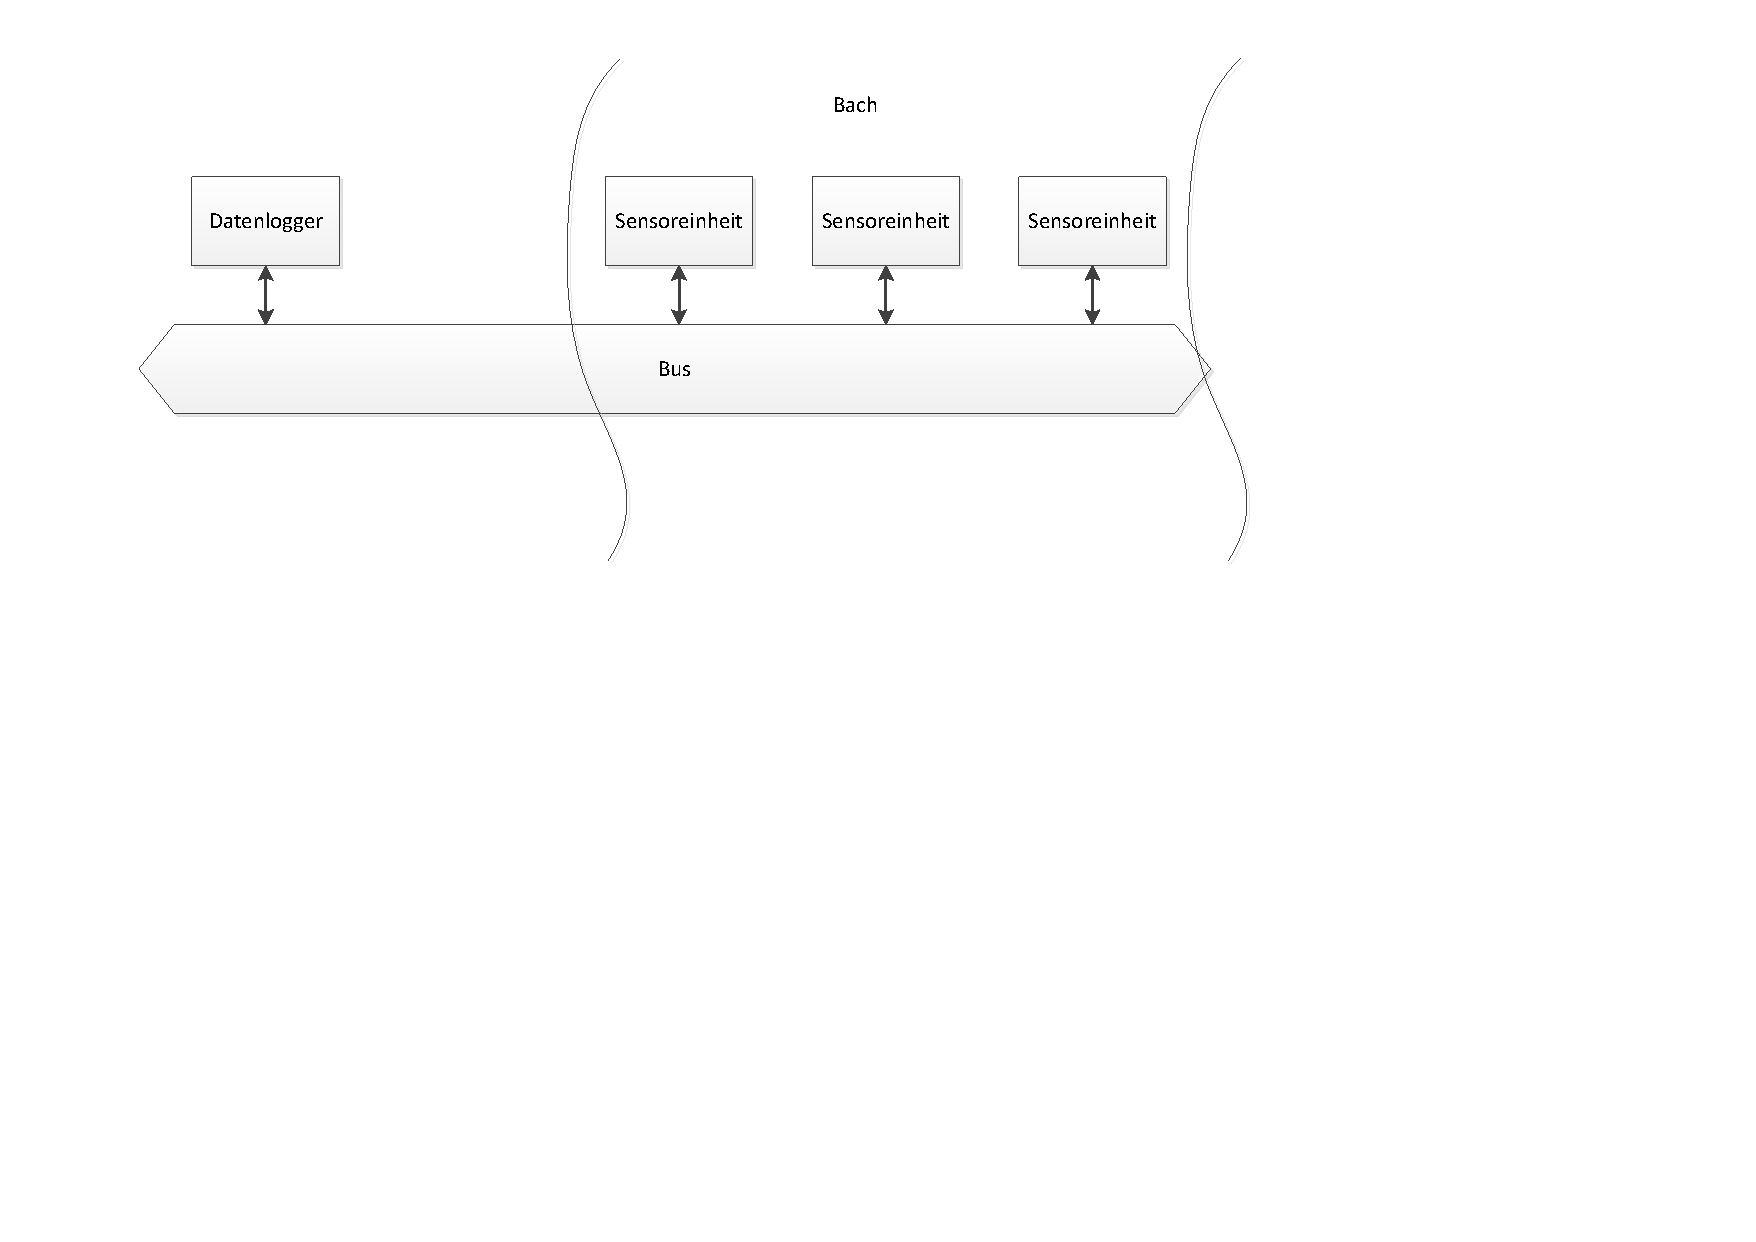
\includegraphics[width=0.8\textwidth]{images/visio/Situationskroki.pdf}
	\caption{Eine Messstation mit einem \gls{logger}, der mehrere \glspl{sensoreinh} im Bach steuert.}
	\label{fig.situationskroki}
\end{figure}

Diese drei Einheiten werden im Folgenden genauer definiert.

\section{Datenlogger}
Der \gls{logger} hat verschiedene Aufgaben zu erfüllen:
\begin{itemize}
\item Sammeln und speichern der Messdaten der \glspl{sensoreinh}.
\item Kontrolle über das \gls{bussys}.
\item Steuerung des Betriebs der Anlage.
\item Schnittstelle für die Konfiguration der Anlage und für das Auslesen der Messdaten.
\end{itemize}


\subsection{Messdaten sammeln}
Für jede angeschlossene \gls{sensoreinh} führt der \gls{logger} eine Datensammlung, in der die registrierten \glspl{ereignis} zeitlich sortiert abgespeichert werden. Die Datensammlungen werden in Dateien abgelegt, die auf einem leicht auswechselbaren Medium abgespeichert werden. So können die Messdaten auf einfache Art für die weitere Auswertung abgeholt werden.


\subsection{Kontrolle über das Bussystem}
Als Busmaster hat der \gls{logger} die Aufgabe, allen angeschlossenen Einheiten eine eindeutige \gls{id} zuzuweisen. Über diese \gls{id} erkennt der \gls{logger}, von welcher \gls{sensoreinh} Daten übertragen werden. Anhand der \gls{id} kann der Datenlogger Konfigurationsnachrichten an bestimmte \glspl{sensoreinh} addressieren. Für die Zuordnung der Messdaten zu einem bestimmten \gls{sensor} benötigen die \glspl{sensoreinh} ein fixes Erkennungsmerkmal, z.B. eine Seriennummer, die mit den Messdaten abgespeichert werden soll. Wurde einer \gls{sensoreinh} einmal eine \gls{id} zugeteilt, wird diese Zugehörigkeit in einer Konfigurationsdatei auf dem \gls{logger} abgespeichert, um bei einem Neustart des Systems die gleichen \gls{id}s zu vergeben.


\subsection{Steuerung des Betriebs}
Die Messstation hat verschiedene \glspl{modus}, die über den \gls{logger} angewählt werden können. Der \gls{logger} steuert die einzelnen \glspl{sensoreinh} entsprechend an. Je nach \gls{modus} weden mehr oder weniger detailreiche Daten über die Ereignisse abgespeichert.


\subsection{Schnittstelle nach Aussen}
Über eine Schnittstelle am \gls{logger} kann ein \gls{compi} angeschlossen werden. Per \gls{cli} wird die Messstation konfiguriert, der Zustand überprüft und der \gls{modus} gewählt.


\section{Sensoreinheit}
Die Aufgaben der \gls{sensoreinh} umfassen:
\begin{itemize}
\item Erfassung von Messdaten.
\item Erkennung von \glspl{ereignis}n.
\item Übertragung der Ereignisdaten an den \gls{logger}.
\end{itemize}


\subsection{Messdatenerfassung}
Der \gls{sensor} zur Erfassung der Daten wird mit einer vordefinierten Abtastrate ausgelesen. Die Abtastrate muss so gewählt werden, dass einzelne \glspl{ereignis} erkannt werden können, ohne unnötig viel Messdaten zu generieren.

\subsection{Ereigniserkennung}
Im Mikroprozessor werden die Messdaten fortlaufend analysiert. Überschreitet das gemessene Signal einen gewissen Schwellenwert (\gls{threshold}), markiert dies den Beginn eines \gls{ereignis}ses. Das \gls{ereignis} ist beendet, wenn der Signalpegel für eine gewisse Zeit (\gls{timeout}) unterhalb des \gls{threshold} bleibt. Für jedes \gls{ereignis} wird abgespeichert, wann es aufgetreten ist (\gls{timestamp}), wie lange es gedauert hat, wie hoch der Signalpegel maximal ausschlug und wie viele Signalspitzen (\glspl{peak}) aufgetreten sind. Allenfalls können auch die Höhen und \glspl{timestamp} aller \glspl{peak} übertragen werden.

\subsection{Datenübertragung}
Die \gls{sensoreinh} sendet die Messdaten regelmässig über das \gls{bussys} an den \gls{logger}. Nach Bestätigung des Erhalts werden die Messdaten aus dem Speicher der \gls{sensoreinh} gelöscht.

\section{Bussystem}
Das \gls{bussys} verbindet die Einheiten der Messstation miteinander. Die gesamten Messdaten und Steuerkommandos werden über den Bus übertragen. Das \gls{bussys} muss die Datenmenge der angeschlossenen \glspl{sensor} bewältigen können, über die geforderte Distanz funktionieren und möglichst robust gegenüber äusseren Einflüssen sein. Der Busmaster hat die Möglichkeit, laufende Übertragungen von \glspl{sensoreinh} zu unterbrechen, um Steuerkommandos zu senden.